\documentclass[a4paper, titlepage]{article}

% For equations
\usepackage{amsmath}

% For including figures
\usepackage{graphicx}

% For typesetting matlab
\usepackage{listings}
\usepackage{color} %red, green, blue, yellow, cyan, magenta, black, white
\definecolor{mygreen}{RGB}{28,172,0} % color values Red, Green, Blue
\definecolor{mylilas}{RGB}{170,55,241}

\lstset{language=Matlab,%
    %basicstyle=\color{red},
    breaklines=true,%
    morekeywords={matlab2tikz},
    keywordstyle=\color{blue},%
    morekeywords=[2]{1}, keywordstyle=[2]{\color{black}},
    identifierstyle=\color{black},%
    stringstyle=\color{mylilas},
    commentstyle=\color{mygreen},%
    showstringspaces=false,%without this there will be a symbol in the places where there is a space
    numbers=left,%
    numberstyle={\tiny \color{black}},% size of the numbers
    numbersep=9pt, % this defines how far the numbers are from the text
    emph=[1]{for,end,break},emphstyle=[1]\color{red}, %some words to emphasise
    %emph=[2]{word1,word2}, emphstyle=[2]{style},    
}


\title{Assignment 1\\
System description and analysis\\
\large EEA004}
\author{Dan Thilderkvist, Philip Gutierrez}

\begin{document}

\maketitle

\section{Background/Introduction}
This assignment study an air handling system with a heater and a humidifier, figure \ref{fig:airSystem}.
The system allow control of two variables, temperature $y_1$ and humidity $y_2$.
This can be done through the flow of of a heater $u_1$ and the flow of a humidifier $u_2$.

\begin{figure}[h!]
\center
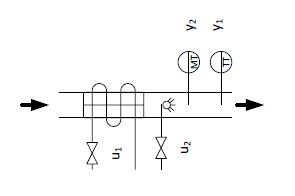
\includegraphics[scale=1]{../figures/heaterHumidifier.png}
\caption{Air management system with heater $u_1$, humidifier $u_2$, thermometer $y_1$ and hygrometer $y_2$.}
\label{fig:airSystem}
\end{figure}

Although the system is not linear, it is assumed linear within a small region of operation.
With this in mind both the heater and the humidifier can be modeled as first order systems, [\ref{equ:firstOrder}].

\begin{equation}
G(s) = \frac{K}{\tau s + 1}
\label{equ:firstOrder}
\end{equation}

The time constant $\tau$ has been given for the heater $\tau_1=50$ and for the humidifier $\tau_2=10$ in the assignment.
The static gain $K$ will have to be calculated for each system.
For that purpose the assignment include two enthalpy–entropy charts, one for each system.
There is also information provided how the system reacts to a step input of $u_1 = 1$ or $u_2 = 2$.
The heater open fully $u_1 = 1$ will increase incoming air of $10^\circ C, 40\% \: RH$ by $15^\circ C$ and the humidifier open fully will increase incoming air of $20^\circ C, 10\% \: RH$ by $70\% \: RH$.

\subsection{Theory}
A linear system can be represented on state space form.
The general form of a state space formulation is as follows:

\begin{equation}
\begin{split}
\dot{x} &= Ax + Bu \\
y &= Cx + Du
\end{split}
\label{equ:stateSpace}
\end{equation}


The final value theorem is something that is often used for system identification.
It can especially come in handy when a system is exited by a step input and the steady state output after a long time can be measured.
The final value theorem states:

\begin{equation}
\lim_{t \to \infty} f(t) = \lim_{s \to 0} sF(s)
\label{equ:finalTheorem}
\end{equation}

Observability of a system loosely indicate if the system states can be reconstructed from the output, if a system is observable the observer poles can be placed arbitrarily.
The observability matrix is defined as such:

\begin{equation}
\mathcal{O}(A,C) = 
\begin{pmatrix}
C \\ CA \\ \vdots \\ CA^{n-1}
\end{pmatrix}
\label{equ:observ}
\end{equation}

If the observability matrix $\mathcal{O}$ has full rank (independent rows/columns) the system is observable.
In a similar fashion, controllability loosely indicate if all states of a system can be controlled by the input, if a system is controllable the poles of a state feedback controller can be arbitrarily chosen.
The Controllability matrix is defined as such:

\begin{equation}
\mathcal{S}(A,B) = 
\begin{pmatrix}
B & AB & \cdots & A^{n-1}C
\end{pmatrix}
\label{equ:contr}
\end{equation}

If the controllability matrix $\mathcal{S}$ has full rank (independent rows/columns) the system is controllable.

When analyzing closed loop systems, not only is the closed loop transfer function $G_c$ of interest, but also a few other functions.
These other functions are related to output stability via noise, disturbance and modeling errors.
They are the sensitivity function $S$, the complementary sensitivity function $T$ and the input sensitivity function $S_u$.
They are defined as follow:

\begin{equation}
\begin{split}
G_c &= (I + GL_y)^{-1}GL_r \\
S &= (I + GL_y)^{-1} \\
T &= (I + GL_y)^{-1}GL_y \\
S_u &= (I + L_yG)^{-1}
\end{split}
\label{equ:transFunc}
\end{equation}

Here $L_y$ is the feedback controller and $L_r$ the feedforward controller of the standard controller form.

\section{Method}
This section will describe the work flow of identifying the air handling system, doing basic analysis on the identified system and in the end designing a controller for for it.

\subsection{System identification}
The air handling system described in the introduction is one of multiple input multiple output (MIMO).
Such a system will have a transfer function matrix $\boldsymbol{G}(s)$ from input to output. In this particular case it will be a $2x2$ matrix because of the two input $u_1, u_2$ and the two output $y_1, y_2$.
The system can be written as such:

\begin{equation}
\begin{split}
\boldsymbol{Y}(s) &= \boldsymbol{G}(s)\boldsymbol{U}(s) \leftrightarrow \\
\begin{pmatrix}
Y_1 \\ Y_2
\end{pmatrix}
&=
\begin{pmatrix}
G_{11}(s) & G_{12}(s) \\ G_{21}(s) & G_{22}(s)
\end{pmatrix}
\begin{pmatrix}
U_1(s) \\ U_2(s)
\end{pmatrix}
\end{split}
\end{equation}

Both heater and humidifier is apporximated by first order systems [\ref{equ:firstOrder}].
Hence the transfer function elements can be written:

\begin{equation}
G_{ij}(s) = \frac{K_{ij}}{\tau_{ij} s + 1}
\end{equation}

Where $\tau_{11} = \tau_{12} = \tau_1 = 50$ and $\tau_{21} = \tau_{22} = \tau_2 = 10$ are given by the assignment and presented in the introduction.

In order to find $K_{ij}$ the final value theorem [\ref{equ:finalTheorem}] can be applied along with the steady state information from the introduction.

\begin{equation}
\begin{split}
\lim_{t \to \infty} y_{1}(t) &= 
\lim_{s \to 0} sY_{1}(s) = 
\lim_{s \to 0} s(G_{11}(s)U_{1}(s) + G_{12}(s)U_{2}(s)) \\
\lim_{t \to \infty} y_{2}(t) &= 
\lim_{s \to 0} sY_{2}(s) = 
\lim_{s \to 0} s(G_{21}(s)U_{1}(s) + G_{22}(s)U_{2}(s))
\end{split}
\label{equ:finalUsage}
\end{equation}

If the input $u(t)$ is a unit step function $l(t)$, the transfer function $U(s)$ is $\frac{1}{s}$ and if only one of $u_1(t)/u_2(t)$ is a step and the other is zero, one of the terms on the right hand side of equation [\ref{equ:finalUsage}] will disappear.
This will render 2 scenarios for the 2 equations:

\begin{equation}
\begin{split}
\lim_{t \to \infty} y_{1}(t) &= 
\lim_{s \to 0} G_{11}(s) = G_{11}(0) = K_{11}, 
\begin{cases}
 u_1(t) = l(t) \\ u_2(t) = 0 
\end{cases} \\
\lim_{t \to \infty} y_{2}(t) &= 
\lim_{s \to 0} G_{21}(s) = G_{21}(0) = K_{21}, 
\begin{cases}
 u_1(t) = l(t) \\ u_2(t) = 0 
\end{cases} \\
\lim_{t \to \infty} y_{1}(t) &= 
\lim_{s \to 0} G_{12}(s) = G_{12}(0) = K_{12}, 
\begin{cases}
 u_1(t) = 0 \\ u_2(t) = l(t) 
\end{cases} \\
\lim_{t \to \infty} y_{2}(t) &= 
\lim_{s \to 0} G_{22}(s) = G_{22}(0) = K_{22}, 
\begin{cases}
 u_1(t) = 0 \\ u_2(t) = l(t) 
\end{cases} \\
\end{split}
\end{equation}

A step input on only one input correspond to the excitation described in the assignment and was presented in the introduction of this report.
The output after such a step input was also given and correspond to the output to 2 of the 4 equations.
The other 2 output can be found using an entropy-enthalpy chart and can be seen in figure \ref{fig:entropy}.
Here the step input effect on the heater (red) and the water mist humidifier (green) can be seen.
The water humidifier was chosen in favor of the steam humidifier as the assignment didn't specify which to use.

\begin{figure}
\center
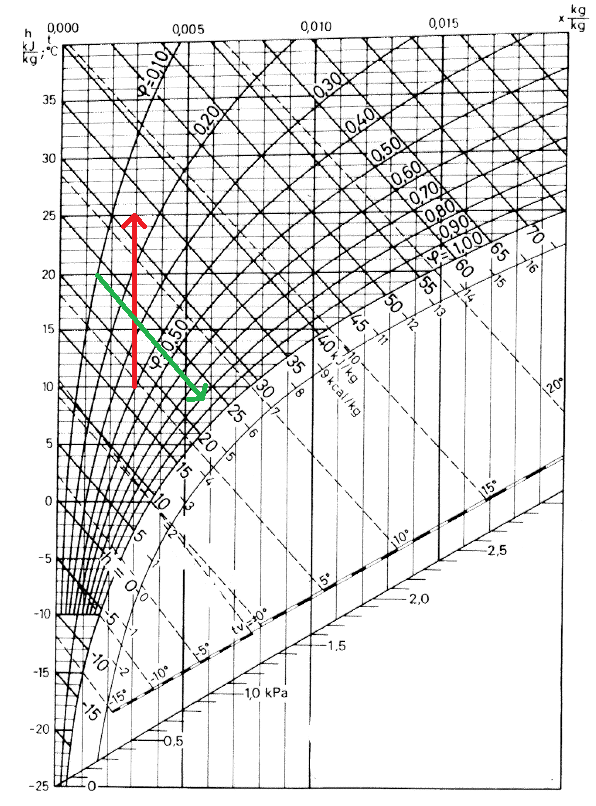
\includegraphics[scale=0.7]{../figures/enthalpyEntropy.png}
\caption{Temperature and humidity effect of a heater step input (red) and of a humidifier step input (green).}
\label{fig:entropy}
\end{figure}

Reading out the temperature and humidity values of the chart give the final static values of the left hand side of equation [\ref{equ:finalUsage}].

\begin{equation}
\begin{split}
25 - 10 = 15 &= 
\lim_{t \to \infty} y_{1}(t) = 
K_{11} \\
15 - 40 = -25 &= 
\lim_{t \to \infty} y_{2}(t) = 
K_{21} \\
9 - 20 = -11 &= 
\lim_{t \to \infty} y_{1}(t) = 
K_{12} \\
80 - 10 = 70 &= 
\lim_{t \to \infty} y_{2}(t) = 
K_{22} \\
\end{split}
\end{equation}

With the values found for $K_{ij}$ and $\tau_{ij}$ the full MIMO system transfer function $\boldsymbol{G}(s)$ can be assembled and is presented in results as equation [input reference to result].

\subsection{System state space formulation}
A linear MIMO system such as the one developed in the previous example can also be expressed on state space form [\ref{equ:stateSpace}].
A simple way to do this is to take aid of a computer.
Matlab offer this functionality through the function \verb|ss(tf)|.
The resulting state space formulation of our system is presented under results as equation [\ref{equ:ssSolution}]

\subsection{Plant model singular values}
The singular values $\sigma_i$ of a MIMO system on state space form [\ref{equ:stateSpace}] are the square roots of the eigenvalues $\sqrt{\lambda_i}$ of the matrix $A^*A$.
The singular values is a measurement of the gain of the system and the input amplification lies between the largest and smallest singular value.
Hence plotting the minimum and maximum singular values for all frequencies correspond to the MIMO equivalent of the bode gain plot.
Since this is tedious to do by hand Matlab offer the function \verb|sigma(G)| to this purpose.
The singular value plot for the air handling system can be found under results as figure [reference figure].

\subsection{System observability and controllability}
For the air handling system the observability and controllability matrices [\ref{equ:observ}],[\ref{equ:contr}] can be calculated using the Matlab commands \verb|obsv(A,C)| and \verb|ctrb(A,B)|.
The matrices for the air handling system are:

\begin{equation}
\mathcal{O} = 
\begin{pmatrix}
0.3 & -0.275		\\
-0.5 & 1.75		\\
-0.006 & 0.0275	\\
0.01 & -0.175
\end{pmatrix}
,\;
\mathcal{C} = 
\begin{pmatrix}
1 & 0 & -0.02 & 0 \\
0 & 4 & 0 & -0.4
\end{pmatrix}
\end{equation}

Using Matlab again \verb|rank(A)| provides the rank of these matrices.
The rank of them can then be compared to the smaller of column count or row count to see if the matrices are full rank.
If they both are full rank the plant is both observable and controllable.

\subsection{Controller design}
A controller $u(t)$ will be designed for the system using feedback.
The general form of a controller is:

\begin{equation}
u(t) = -K_y(p)y(t) + K_r(p)r(t)
\end{equation}

The assignment asks for a standard proportional controller on each output.
For a standard proportional controller $K_r = K_y$ and the proportional gains $k_{p,i}$ will be the diagonal of the controller matrix $K_y$.
With 2 system outputs, 2 control signals and 2 reference values the size of $K_y$ will be a $2 \times 2$ matrix.
For the air handling system with proportional controller feedback the controller will be:

\begin{equation}
\begin{split}
u(t) = -K_y(p)y(t) + K_y(p)r(t) &= 
K_y(p)(-y(t) + r(t)) = 
K_y(p)e(t) \\
K_y(p) &= 
\begin{pmatrix}
k_{p,1} 	& 	0 		\\
0 		&	k_{p,2}	
\end{pmatrix}
\end{split}
\end{equation}

The gain values $k_{p,i}$ are selected in 3 different interesting combinations, shown in table \ref{tab:gains}.

\begin{table}[h!]
\begin{center}
\begin{tabular}{||c | c c||}
 \hline
 Test & $k_{p,1}$ & $k_{p,2}$ \\ [0.5ex] 
 \hline\hline
 1 &  1 & 1 \\ 
 \hline
 2 &  1 & 0.1 \\
 \hline
 3 &  5 & 5 \\
 \hline
\end{tabular}
\end{center}
\caption{Controller gains used during evaluation.}
\label{tab:gains}
\end{table}

With the controller defined the stability functions [\ref{equ:transFunc}] can be calculated using Matlab standard matrix operations.
The singular values of the stability functions are then plotted, again using \verb|sigma(F)|, the singular value plots are found in results as figures [reference all singular value plots].

\section{Results}

\subsection{Question 1}

\subsection{Question 2}

\begin{equation}
\begin{split}
\dot{x} &= 
\begin{pmatrix}
-0.02 & 0 \\ 0 & -0.1
\end{pmatrix}x
+
\begin{pmatrix}
0.3 & -0.5 \\ -0.25 & 1.75
\end{pmatrix}u \\
y &= 
\begin{pmatrix}
1 & 0 \\ 0 & 4
\end{pmatrix}x
\end{split}
\label{equ:ssSolution}
\end{equation}

\subsection{Question 3}

\subsection{Question 4}

\subsection{Question 5}

\begin{equation}
U(s) = -L_y(s)Y(s) + L_r(s)R(s) 
\end{equation}



\section{Conclusion/Discussion}


\section{Example code}

\includegraphics[scale=0.8]{../code/figures/exampleFigure.png}

\lstinputlisting{../code/exampleCode.m}

\end{document}